\section{Same side track identification using a Boosted Decision Tree}
\label{sec:SS_classifier}

To identify tracks that belong to the SS of a signal $B$, a BDT is trained on the simulated LHCb data. 
The BDT output resembles a probability of the track being in the SS and is from now on called $\text{Prob}_\text{SS}$.
The implementation of the BDT is done in Python with the library XGBoost \cite{xgboost}.

The dataset used for training the BDT contains about 70 different features on the tracks of the associated event.
To reduce this list of features, first the correlation coefficient between all feature pairs is calculated.
Features with a correlation near $100\%$ are considered to contain redundant information.
Only one feature of each set of highly correlated features is kept for training the BDT.
Next, a BDT is trained on a dataset containing all features and the gain of each feature is calculated.
The gain is a measure used in decision trees to estimate the accuracy improvement of the introduction of a cut on one feature.
Additionally, the permutation importance of the ROC AUC is calculated.
The permutation importance is the difference in any performance metric after making predictions on a dataset with the entries of a single feature permuted at random.
The features with the lowest gain or permutation importance are discarded until a reasonable amount of features is achieved.
The remaining 21 features are listed in \autoref{tab:SS_features} and the corresponding feature importances are shown in \autoref{fig:SS_importances}.

\begin{figure}
    \centering
    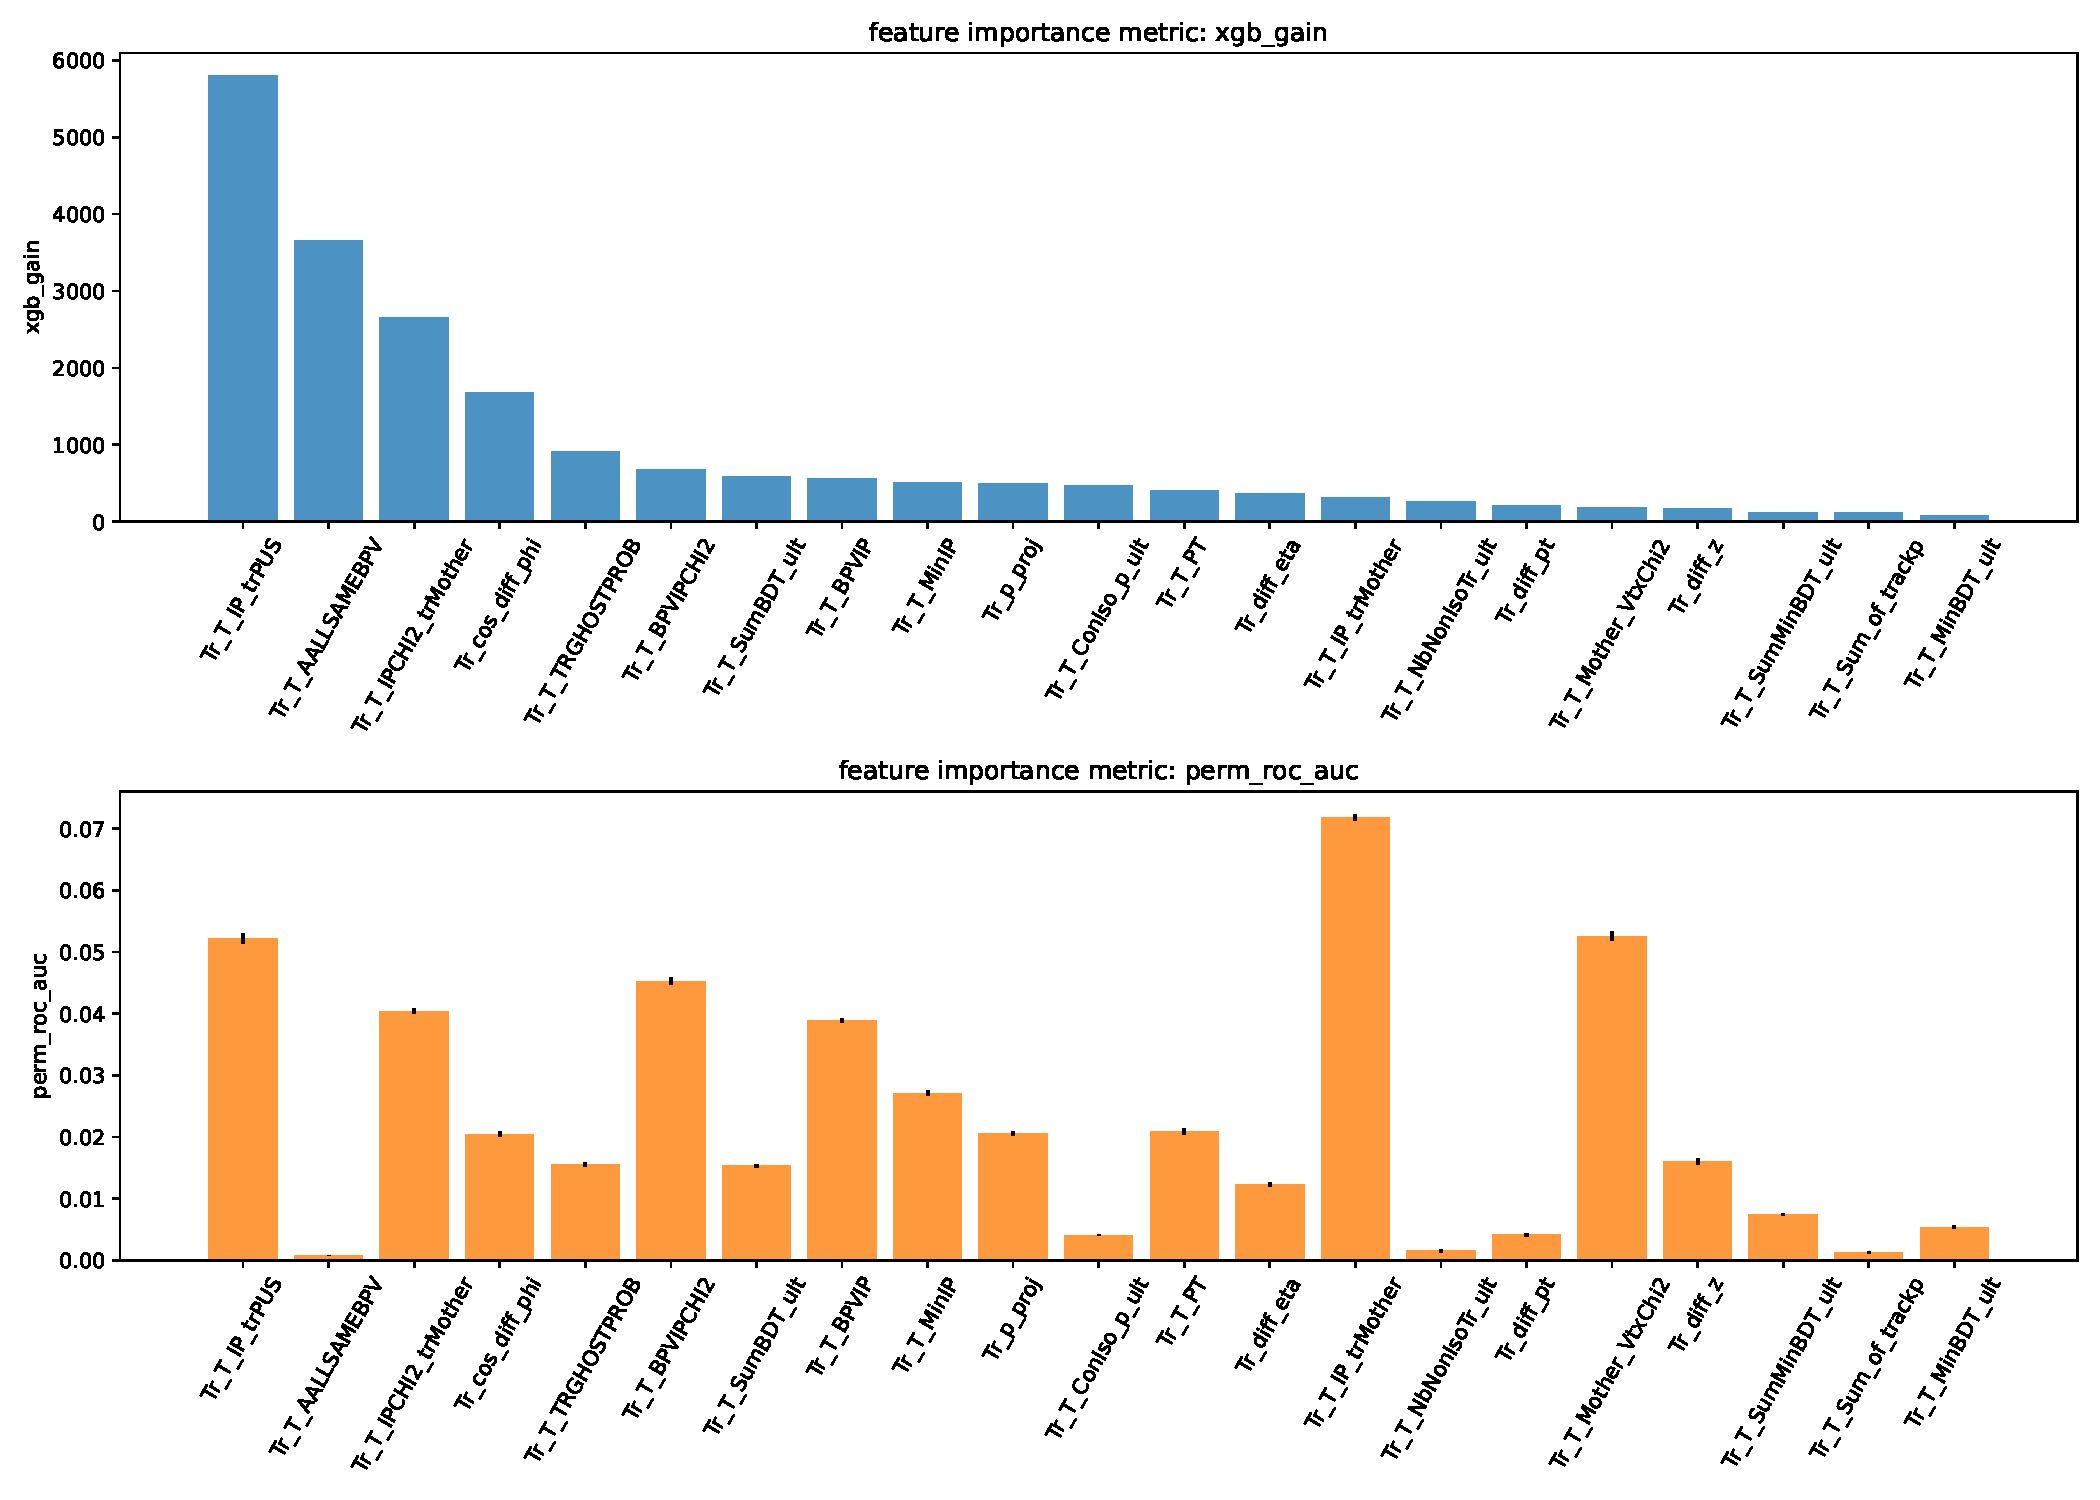
\includegraphics[width=\textwidth]{images/SS_feature_importances.pdf}
    \caption{Calculated feature importances on the trained DeepSet. Shown are the gains and the permutation importances of the ROC AUC.}
    \label{fig:SS_importances}
\end{figure}

\begin{table}
    \centering
    \caption{List of all features used to train the BDT for SS track identification.}
    \label{tab:SS_features}
    \begin{tabular}{c c}
        \toprule
        feature & feature \\
        \midrule
        $p_\text{T}$        & IP\_trMother \\ %"Tr_T_PT","Tr_T_IP_trMother"
        $p_\text{proj}$     & IPCHI2\_trMother \\ %"Tr_p_proj","Tr_T_IPCHI2_trMother"
        $\Delta p_\text{T}$ & IP\_trPUS \\ %"Tr_diff_pt","Tr_T_IP_trPUS"
        $\Delta z$          & MinBDT\_ult \\ %"Tr_diff_z","Tr_T_MinBDT_ult"
        $\Delta \eta$       & Mother\_VtxChi2 \\ %"Tr_diff_eta","Tr_T_Mother_VtxChi2"
        $\cos(\Delta \phi)$ & NbNonIsoTr\_ult \\ %"Tr_cos_diff_phi","Tr_T_NbNonIsoTr_ult"
        AALLSAMEBPV         & SumBDT\_ult \\ %"Tr_T_AALLSAMEBPV","Tr_T_SumBDT_ult"
        BPVIP               & SumMinBDT\_ult \\ %"Tr_T_BPVIP","Tr_T_SumMinBDT_ult"
        $\text{BPVIP}_{\chi^2}$    & Sum\_of\_trackp \\ %"Tr_T_BPVIPCHI2","Tr_T_Sum_of_trackp"
        MinIP               & TRGHOSTPROB \\ %"Tr_T_MinIP","Tr_T_TRGHOSTPROB"
        ConIso\_p\_ult      & \\ %"Tr_T_ConIso_p_ult",
        \bottomrule
    \end{tabular}
\end{table}

(Explain all features)....

Then a BDT is trained on a dataset containing all features of this list.
From the $18$ million tracks in the dataset, $60\%$ are used for training and $40\%$ are used for validation of the trained model.
The trained model contains $2000$ estimators at a maximum decision tree depth of $4$.
The learning rate is set to $0.1$.
Due to the imbalance of SS tracks and other tracks in the data, the parameter \enquote{scale\_pos\_weight} is set to $N_\text{other}/N_\text{SS} = 11.94$.
The learning objective is logistic regression for binary classification.

The negative log-likelihood and the error rate for each iteration of the training of the BDT are shown in \autoref{fig:SS_history}.
The error rate is the proportion of predictions matching the ground truth of the simulation.
For this, all tracks with $\text{Prob}_\text{SS}>0.5$ count as predicted SS tracks. 

\begin{figure}
    \centering
    \begin{subfigure}{0.5\textwidth}
        \centering
        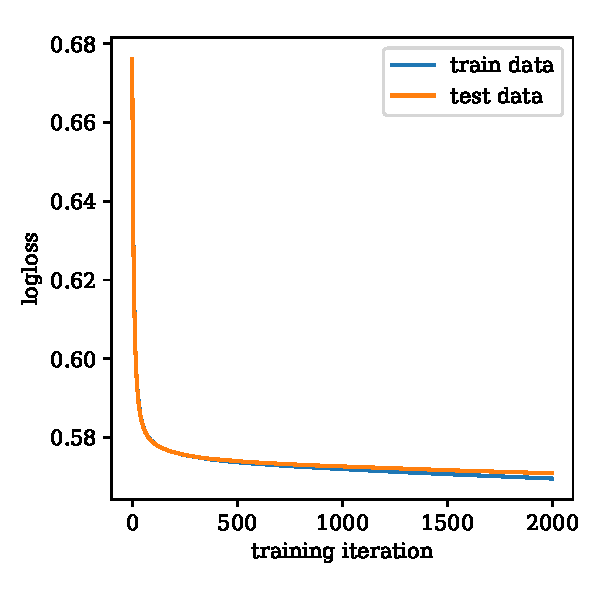
\includegraphics[width=\textwidth]{images/SS_history_logloss.pdf}
        \caption{negative log-likelihood}
    \end{subfigure}%
    \begin{subfigure}{0.5\textwidth}
        \centering
        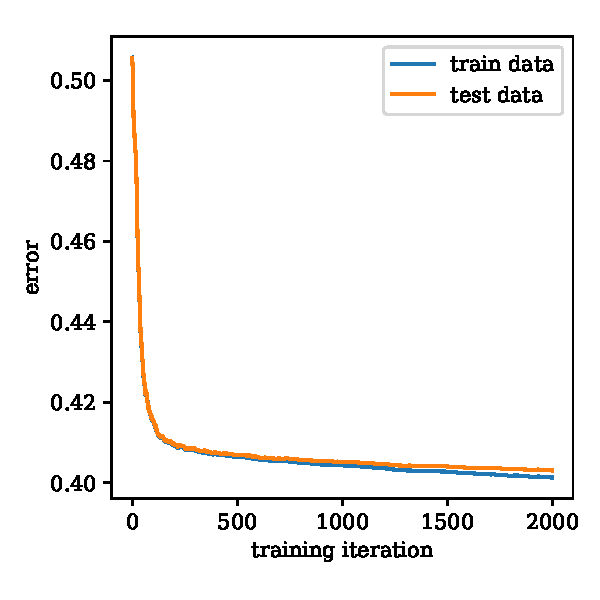
\includegraphics[width=\textwidth]{images/SS_history_error.pdf}
        \caption{error rate}
    \end{subfigure}%
    \caption{Training performance of the SS BDT.}
    \label{fig:SS_history}
\end{figure}

To show the achieved separation of the SS tracks, histograms of $\text{Prob}_\text{SS}$ split by the simulation ground truth are shown in \autoref{fig:SS_output}.
A measure of separation is the ROC (reciever operating characteristic) curve shown in \autoref{fig:SS_ROC}.
The achieved ROC AUC (area under the ROC curve) is $0.763$ on the test data and $0.767$ on the training data.
A ROC AUC of $1.0$ means perfect separation and a ROC AUC of $0.5$ means no separation.
To estimate the generalization and overtraining of the model, each performance measure is calculated on both the test data and training data.

\begin{figure}
    \centering
    \begin{subfigure}{0.5\textwidth}
        \centering
        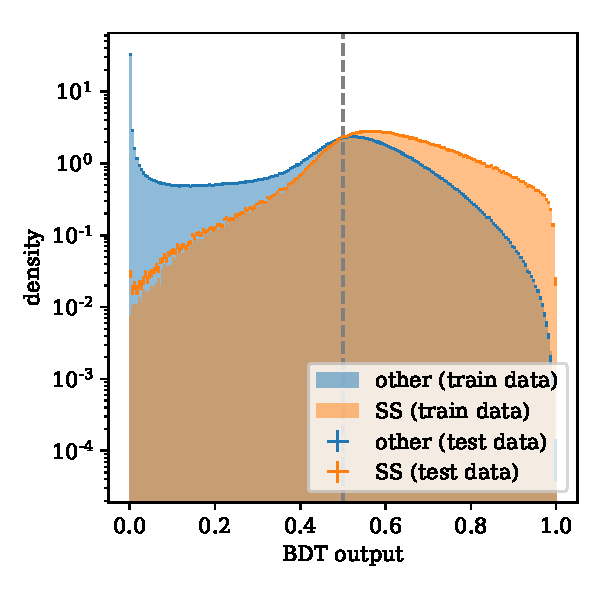
\includegraphics[width=\textwidth]{images/SS_output.pdf}
        \caption{distribution of $\text{Prob}_\text{SS}$}
        \label{fig:SS_output}
    \end{subfigure}%
    \begin{subfigure}{0.5\textwidth}
        \centering
        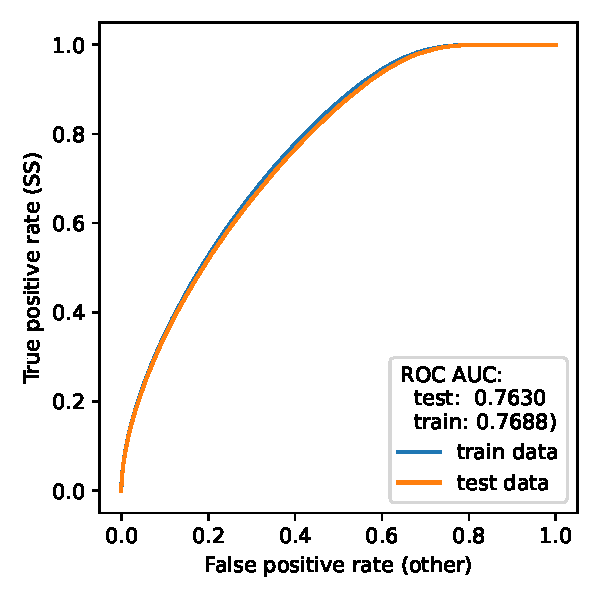
\includegraphics[width=\textwidth]{images/SS_ROC.pdf}
        \caption{ROC curve}
        \label{fig:SS_ROC}
    \end{subfigure}%
    \caption{\autoref{fig:SS_output} shows the distribution of the BDT output split by the simulation ground truth. \autoref{fig:SS_ROC} shows the ROC curve of the BDT output. Both figures show the BDT prediction for the test data and the training data.}
\end{figure}
